% the é for free use
\section{Introduction}
\subsection{Motivation}
Computer Aided Geometrical Design, or CAGD, is a branch of numerical mathematics which has a variety of practical applications.\\
Bézier curves are generally utilized to model smooth curves, especially quadratic or cubic ones. They are defined by control polygons and manipulating these polygons results in a change in the original curve. Thus it is quite simple to adjust Bézier curves, which is why they are widely used in computer design, animations, font design, and the car industry. Indeed, Piere Bézier originally invented them to design curves for the bodywork of Renault cars \cite{10.5555/501891}.\\
Constraint Delaunay triangulations are applied in path planning in automated driving and topographic surveying \cite{6232153} and Voronoi diagrams, which are closely related to Delaunay triangulation, are used in fields like biology to model cell \cite{2009arXiv0901.4469B} or bone structures \cite{2012SPIE.8290E..0PL}. More on that later.

\subsection{Scope of this Project}
The main goal of this project was to implement the various algorithms from chapter 3, 4, and 5 of Gerald Farin's book "Curves and Surfaces for CAGD, a pracitcal guide" using Python. That means each mathematical result and formula is taken from this book unless stated differently. \\
The content of chapter 3 focuses on more fundamental topics like linear interpolation or blossoms and served as a great introduction. The most challenging part of not only this chapter but also the entire project was the implementation of an algorithm for the Delaunay triangulation and also the Voronoi diagram.\\
Chapter 4 serves as an introduction to Bézier curves and describes the de Casteljau algorithm. Furthermore it describes properties of Bézier curves and the technique of blossoming. \\
Chapter 5 expands on these topics as it proposes more variations on how one can compute Bézier curves, for instance subdivision and Bernstein polynomials. Moreover different forms of Bézier curves are introduced, namely the monomial and matrix form from which we only focused on the monomial form. At last more properties like the derivative of Bézier curves are established. We decided to not use the matrix form because of its bad conditioning.\\
Since the book didn't contain any definitions on Voronoi diagrams and Delaunay triangulations, this scope extended. We looked at the current literature, evaluated different algorithmic concepts and implemented a \cite{Green1978} based algorithm. 

The project structure can be seen in Figure 1.
\begin{figure}[H]
\centering
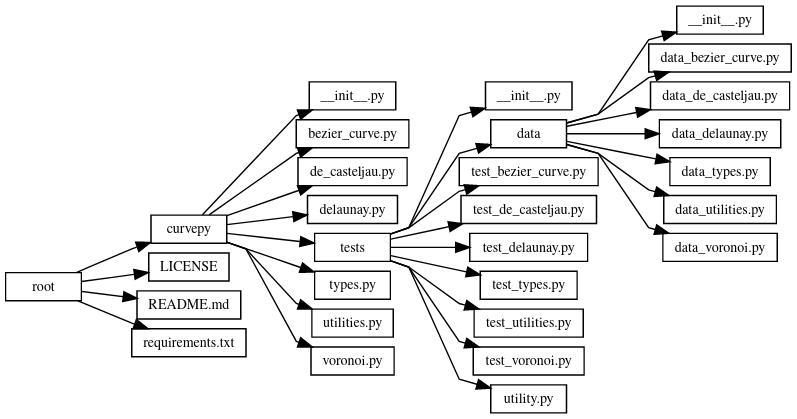
\includegraphics[width=\textwidth]{graphviz.png}
\caption{Project Structure}
\end{figure}
Let us briefly go over the most important architectural design decisions:
\begin{itemize}
    \item[\texttt{requirements.txt}] To keep overhead as minimal as possible we decided to track dependencies via \texttt{requirements.txt} instead of using a more sophisticated build system like \texttt{poetry}.
    \item[\texttt{curvepy}] All Python code is contained within the \texttt{curvepy} top level module, even the tests. This is essential; otherwise any deployment tool (like \texttt{setuptools}) would declare \texttt{tests} as a top level module as well, thus overshadowing any other test module installed within the python environment. Each python file has a has a matching test and data file.
    \item[\texttt{tests}] Our 1000+ test cases, mostly against precomputed and manually verified values contained in \texttt{data}.
    \item[\texttt{\_\_init\_\_.py}] Although most \texttt{\_\_init\_\_.py} files contain no code, they have two specific usages: On the one hand, they contain docstrings which are processed by \texttt{pdoc3} for HTML-documentation. On the other hand, they are required by Python so that the folder is recognized as a module.
    \item[\texttt{LICENSE}] To allow the least restrictive usage of our algorithms, while still keeping ownership of it's interlectual property (unlike public domain licenses like CC-0), we provide all our code as MIT licensed.
    \item[\texttt{README.md}] To provide a simple overview, our library contains a \texttt{README.md}, which can be rendered by Gitlab. 
\end{itemize}
The python files are organized as follows:
\begin{itemize}
    \item[\texttt{bezier\_curve.py}] contains multiple Bézier curve implementations. They all have the same methods; this is done via abstract class inheritance.
    \item[\texttt{de\_casteljau.py}] contains an implementation of the De Casteljau algorithm for computing Bézier curves as well as some utility methods.
    \item[\texttt{delaunay.py}] contains an implementation of a Delaunay triangulation algorithm. It is also used to compute it's dual graph, the Voronoi diagram.
    \item[\texttt{types.py/utilities.py}] contain various helper methods and classes.
    \item[\texttt{voronoi.py}] computes the voronoi diagram through it's underlying Delaunay triangulation.
\end{itemize}
\subsection{Technical Decisions}
Here are some of our technical decisions with their reasoning:
\begin{itemize}
    \item Since we see ourselves as an mostly educational implementation, we formally only support Python 3.8+, although we use \texttt{\_\_future\_\_} imports to keep as much backwards compatibility as possible.\\
    We do not require any complicated version testing tool like \texttt{tox} or building tool like \texttt{poetry}.
    \item Our code style is mostly PEP-8 conform, but with a few exceptions. Here are the according \texttt{flake8}-IDs:
    \begin{itemize}
        \item[\textbf{E731}] \textit{"Do not assign a lambda expression, use a def"}\\
        For single usage methods, we sometimes want to assign a variable name to offer more semantics.
        \item[\textbf{E125}] \textit{"Continuation line with same indent as next logical line"}\\
        This is simply not compatible with PyCharm, which we use as our formatter.
        \item For easier readability, we allow line lengths with up to 120 characters.
    \end{itemize}
    \item For docstrings, we use the \texttt{numpy} docstring format, as we heavily depend on \texttt{numpy} and \texttt{scipy}.
    \item For docstring-based HTML documentation we use \texttt{pdoc3}, since it covers all our use cases while being simpler than sphinx, which requires additional reStructuredText files.
    \item We use \texttt{pytest} for unit tests because it is the most commonly used mature python unit testing framework.
    \item For formatting, we use Jetbrains default formatter, which is shipped with PyCharm.\\
    Additionally, we use \texttt{isort} for import ordering.
    \item Once we publish our library on PyPI, we will use version numbers according to PEP 440.\\
    Note that this is \textit{not} compatible with Semantic Versioning (SemVer).\\
    Further note that this prohibits git-hashes as version numbers since they have no formal ordering.
\end{itemize}
We also use the continuous integration (CI) provided by Gitlab. Specifically, we use the default Gitlab runner provided by the GWDG. Our pipeline is split into 3 stages:
\begin{itemize}
    \item[\texttt{static-analysis}] We use \texttt{flake8} as our linter. \texttt{flake8} is a combination of \texttt{pep8}, which checks conformity against the PEP 8 design standard, as well as \texttt{pyflakes}, which provides a substantial amount of plugin functionality.\\
    We use the following extensions:
    \begin{itemize}
        \item \texttt{flake8-bugbear} "A plugin for Flake8 finding likely bugs and design problems in your program."
        \item \texttt{pep8-naming} "Check your code against PEP 8 naming conventions."
        \item \texttt{flake8-builtins} "Check for python builtins being used as variables or parameters."
        \item \texttt{flake8-comprehensions} "A flake8 plugin that helps you write better list/set/dict comprehensions."
    \end{itemize}
    \item[\texttt{test}] On every commit to \texttt{master} as well as merge requests we run our full \texttt{pytest} based test suite.
    \item[\texttt{deploy}] After every commit to \texttt{master}, we automatically update and redeploy our HTML based documentation \cite{CPY}.
\end{itemize}
\subsection{Acknowledgements}
Firstly, we want to thank Dr. Jochen Schulz and Prof. Dr. Gerlind Plonka-Hoch for their monumental patience, waiting around 2 years for this project to complete.\\
Secondly, we want to thank Gerald E. Farin for his detailed overview of computer aided graphic design \cite{10.5555/501891} and Franz Aurenhammer and Steven Fortune for their great meta analysis of Voronoi and Delaunay research \cite{Aurenhammer1991} \cite{FORTUNE1995}.\\
Lastly, we want to thank the now defunct "Coffeebar ins Grüne" for all the great Currywursts which were soaked in a comically large amount of oil that would make any government jealous.